\begin{figure*}[t]
    \centering
    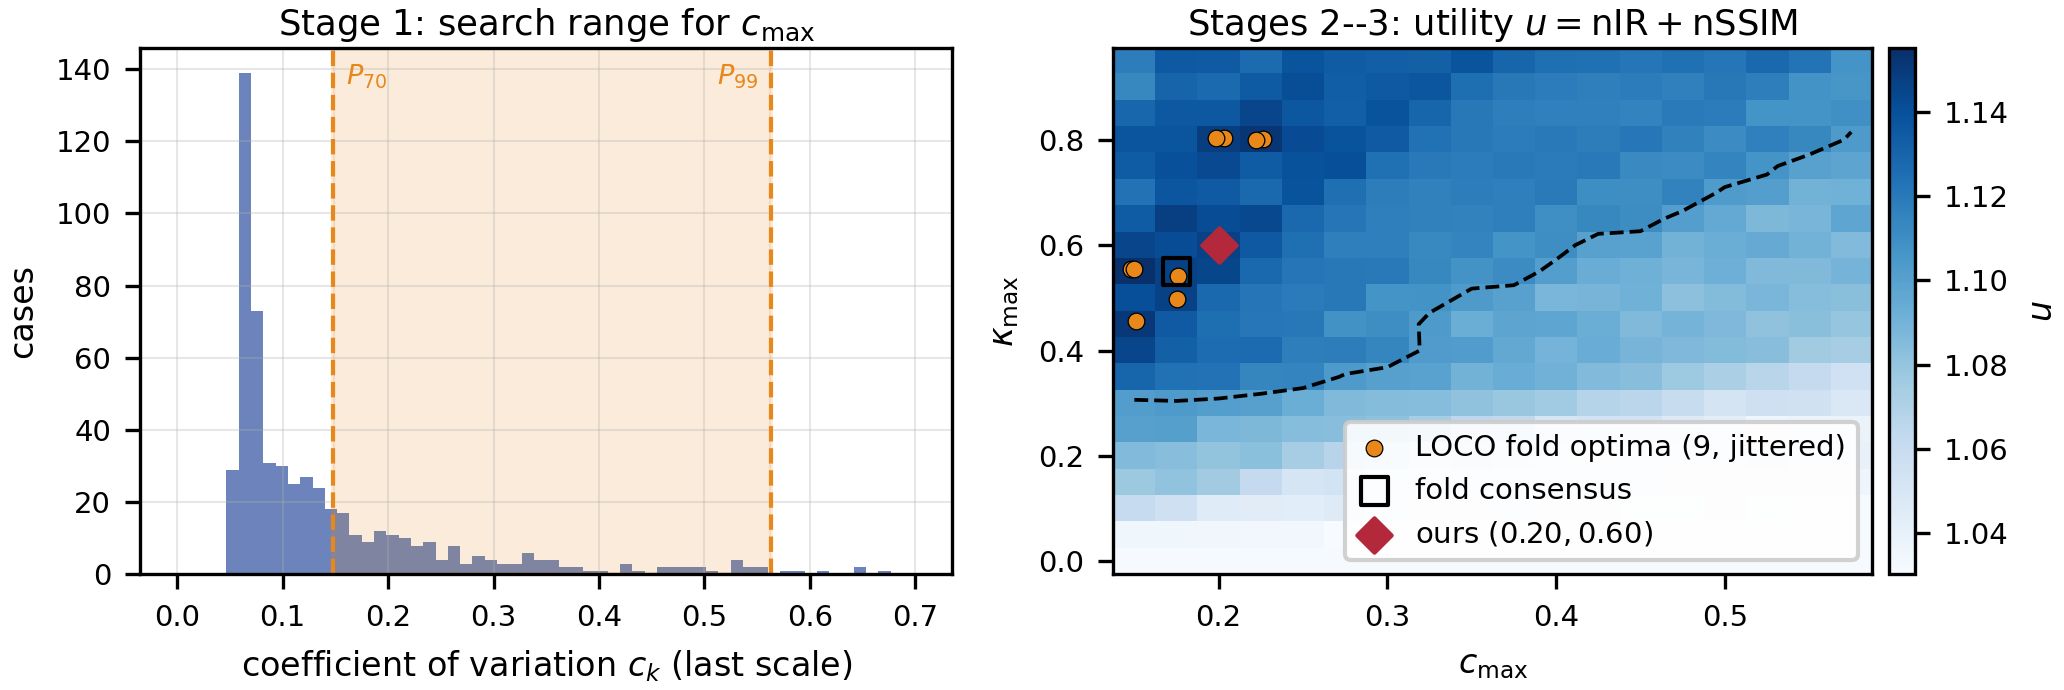
\includegraphics[width=\textwidth]{imgs/fig_protocol.png}
    \caption{Parameter selection. \textbf{Left:} Stage 1 derives the search range for $c_{\max}$ from the dev-set distribution of $c_k$ rather than by hand --- below $P_{70}$ more than half the cases are clamped at $\kappa_{\max}$ and the mapping stops discriminating, above $P_{99}$ nothing is clamped and it degenerates to a linear ramp. \textbf{Right:} the composite utility $u = \mathrm{nIR} + \mathrm{nSSIM}$ over the resulting $18 \times 20$ grid. The dashed contour bounds the flat region ($u \ge u_{\max} - 0.05$), which covers 45\% of the grid; all nine leave-one-category-out optima fall inside it, and the parameters used in this paper sit $\Delta u = 0.008$ from the grid optimum. Utility decreases sharply only towards small $\kappa_{\max}$ (bottom band), i.e.\ the adaptive term has to be given enough range to contribute.}
    \label{fig:protocol}
\end{figure*}
